\chapter{Beyond Variance Reduction: Understanding the True Impact of Baselines on Policy Optimization}
\label{chapter:baselines}
\section*{Article details}
Thomas Valentin*, Chung Wesley*, Machado Marlos C., Le Roux Nicolas ``Beyond variance reduction: Understanding the true impact of baselines on policy optimization''. In \emph{International Conference on Machine Learning (ICML) 2021. PMLR}.

\section*{Foreword}
In the summer of 2019, I interned at Google Brain Montr\'{e}al with Nicolas Le Roux and Marlos C. Machado and my project was initially about using off-policy learning to reduce the variance of the gradients for Policy Gradient methods in Reinforcement Learning. However, when comparing our method to other variance reduction methods, such as the use of baselines, I came to realise that \emph{symmetric} perturbations of the variance-minimizing baseline (e.g $\pm \epsilon$), while increasing the variance by the same amount, led to \emph{asymmetric} impacts on the regret/average reward. While we initially decided to continue exploring the first project, we came back to this observation which Wesley had begun to work on with Nicolas. By studying this on simple examples such as a two-arm bandits, Nicolas was first able to demonstrate our first divergence result. During the year 2020, we worked together on extending both the divergence and convergence results and deepened our understanding of the problem.

This paper could be described as one pointing out a surprising flaw in a widely used algorithm and as such it inspired future work. The most relevant direct line of work inspired by our article is the one led by Jincheng Mei who worked previously on the convergence of policy gradient methods in the \emph{expected} regime. 

\section*{Impact since publication}
Following our work, \citet{mei2021understanding} extended our observation to a vast class of algorithms: those which are too greedy, or \emph{committal} and may converge prematurely to a suboptimal solution. Finally, we (Jincheng, Wesley and I) started collaborating together and this culminated in a paper \emph{The Role of Baselines in Policy Optimization}~\citep{mei2022role} published at NeurIPS 2022 which sheds light on how baselines impact the exploration behavior of policy gradient methods and how using the value function as a baseline guarantees policy improvement in expectation while the variance-minimizing baseline may not. As such policy gradient using the true value function as a baseline can converge to the optimal policy fast.


\section*{Personal contribution}
\begin{itemize}
    \item The original observation that baselines impact not only the variance but also the convergence of Policy Gradient methods was done by me during my summer internship at Google Brain with Nicolas and Marlos
    \item Theory (convergence proofs) and experiments for the off-policy setting with the collaboration of Wesley for the extension to $K > 2$ arms
    \item Collaboration with Wesley on the divergence proofs for the 3 arms setting
    \item Design of the simplex visualizations (\Cref{fig:trajectories} and \Cref{fig:simplex_variance})
    \item Writing of the paper alongside with all my co-authors
\end{itemize}



\begin{abstract}


Bandit and reinforcement learning (RL) problems can often be framed as optimization problems where the goal is to maximize average performance while having access only to stochastic estimates of the true gradient. Traditionally, stochastic optimization theory predicts that learning dynamics are governed by the curvature of the loss function and the noise of the gradient estimates. In this paper we demonstrate that the standard view is too limited for bandit and RL problems. To allow our analysis to be interpreted in light of multi-step MDPs, we focus on techniques derived from stochastic optimization principles~(e.g., natural policy gradient and EXP3) and we show that some standard assumptions from optimization theory are violated in these problems. We present theoretical results showing that, at least for bandit problems, curvature and noise are not sufficient to explain the learning dynamics and that seemingly innocuous choices like the baseline can determine whether an algorithm converges. These theoretical findings match our empirical evaluation, which we extend to multi-state MDPs.
\end{abstract}

\section{Introduction}
In the standard multi-arm bandit setting~\cite{robbins1952some}, an agent needs to choose, at each timestep $t$, an arm $a_t \in \{1, ..., n\}$ to play, receiving a potentially stochastic reward $r_t$ with mean $\mu_{a_t}$. The goal of the agent is usually to maximize the total sum of rewards, $\sum_{i=1}^T r_i$, or to maximize the average performance at time $T$, $\E_{i\sim \pi} \mu_i$ with $\pi$ being the probability of the agent of drawing each arm~\citep{bubeck2012regret}. While the former measure is often used in the context of bandits,\footnote{The objective is usually presented as regret minimization.} $\E_{i\sim \pi} \mu_i$ is more common in the context of Markov Decision Processes (MDPs), which have multi-arm bandits as a special case.

In this paper we focus on techniques derived from stochastic optimization principles, such as EXP3~\citep{auer2002nonstochastic, seldin2013evaluation}. %
In particular, we study \textit{policy gradient} methods, a family of algorithms useful in the more general MDP setting which have seen empirical success in recent times \cite{schulman2017proximal}. 


We analyze the problem of learning to maximize the average reward, $\gJ$, by gradient ascent:
\begin{align}
    \theta^\ast &= \arg\max_\theta \gJ(\theta)
    = \arg\max_\theta \sum_{a} \pi_\theta(a) \mu_a \; , \label{eq:bandit_loss} 
\end{align} 
with $\mu_a$ being the average reward of arm $a$.
In this case, we are mainly interested in outputting an effective policy at the end of the optimization process, without explicitly considering the performance of intermediary policies.%


Optimization theory predicts that the convergence speed of stochastic gradient methods will be affected by the variance of the gradient estimates and by the geometry of the function $\gJ$, represented by its curvature. Roughly speaking, the geometry dictates how effective true gradient ascent is at optimizing $\gJ(\theta)$ while the variance can be viewed as a penalty, capturing how much slower the optimization process is by using noisy versions of this true gradient. More concretely, doing one gradient step with stepsize $\alpha$, using a stochastic estimate $g_t$ of the gradient, leads to \citep{bottou2018optimization}:
\begin{align*}\E[\gJ(\theta_{t+1})] - \gJ(\theta_t) &\geq (\alpha - \tfrac{L \alpha^2}{2}) \|\E [g_t] \|^2_2  - \tfrac{ L \alpha^2}{2} \text{Var}[g_t ],\end{align*}
when $\gJ$ is $L$-smooth, i.e. its gradients are $L$-Lipschitz. 

As large variance has been identified as an issue for policy gradient (PG) methods, many works have focused on reducing the noise of the updates. One common technique is the use of control variates~\citep{greensmith2004variance, hofmann2015variance}, referred to as \emph{baselines} in the context of RL. These baselines $b$ are subtracted from the observed returns to obtain shifted returns, $r(a_i) - b$, and do not change the expectation of the gradient. In MDPs, they are typically state-dependent.
While the value function is a common choice, previous work showed that the minimum-variance baseline for the REINFORCE \citep{williams1992simple} estimator is different and involves the norm of the gradient~\citep{peters2008reinforcement}.
Reducing variance has been the main motivation for many previous works on baselines~\citep[e.g.,][]{gu2016q, liu2017action, grathwohl2017backpropagation, wu2018variance, cheng2020trajectory}, but the influence of baselines on other aspects of the optimization process has hardly been studied. We take a deeper look at baselines and their effects on optimization.

\subsubsection*{Contributions}
We show that baselines can impact the optimization process 
beyond variance reduction and lead to qualitatively different learning curves, even when the variance of the gradients is the same. 
For instance, given two baselines with the same variance, the more negative baseline promotes \textit{committal} behaviour where a policy quickly tends towards a deterministic one, while the more positive baseline leads to \textit{non-committal} behaviour, where the policy retains higher entropy for a longer period.

Furthermore, we show that \textbf{the choice of baseline can even impact the convergence of natural policy gradient} (NPG), something variance cannot explain. In particular, we construct a three-armed bandit where using the baseline minimizing the variance can lead to convergence to a deterministic, sub-optimal policy for any positive stepsize, while another baseline, with larger variance, guarantees convergence to the optimal policy. As such a behaviour is impossible under the standard assumptions in optimization, this result shows how these assumptions may be violated in practice. It also provides a counterexample to the convergence of NPG algorithms in general, a popular variant with much faster convergence rates than vanilla PG when using the true gradient in tabular MDPs~\citep{agarwal2019optimality}. 

Further, \textbf{we identify on-policy sampling as a key factor to these convergence issues} as it induces a vicious cycle where making bad updates can lead to worse policies, in turn leading to worse updates. A natural solution is to break the dependency between the sampling distribution and the updates through off-policy sampling. We show that ensuring all actions are sampled with sufficiently large probability at each step is enough to guarantee convergence in probability. Note that this form of convergence is stronger than convergence of the expected iterates, a more common type of result \citep[e.g.,][]{mei2020global,agarwal2019optimality}.

We also perform an empirical evaluation on multi-step MDPs, showing that baselines have a similar impact in that setting. We observe \textbf{a significant impact on the empirical performance} of agents when using two different sets of baselines yielding the same variance, once again suggesting that learning dynamics in MDPs are governed by more than the curvature of the loss and the variance of the gradients.



\begin{figure*}[t]
\label{fig:npg_simplex}
\centering
  \begin{subfigure}[b]{0.24\linewidth}
    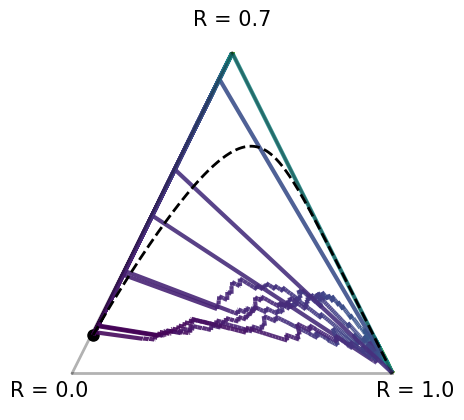
\includegraphics[width=\textwidth]{articles/baselines/figs/reproduced_simplex_npg/natural_minvar_-05.png}
    \caption{$b^-_\theta = b^*_\theta - \nicefrac{1}{2} $}
    \label{fig:-1}
  \end{subfigure}
  \hfill
    \begin{subfigure}[b]{0.24\linewidth}
    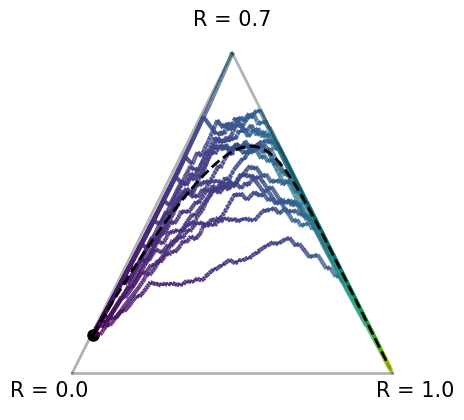
\includegraphics[width=\textwidth]{articles/baselines/figs/reproduced_simplex_npg/natural_minvar_00.png}
    \caption{$b_\theta = b^*_\theta$}
    \label{fig:0}
  \end{subfigure}
  \hfill
  \begin{subfigure}[b]{0.24\linewidth}
    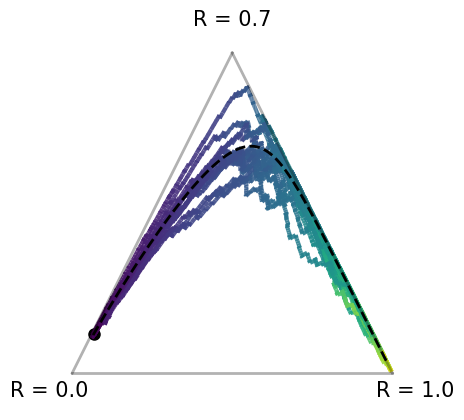
\includegraphics[width=\textwidth]{articles/baselines/figs/reproduced_simplex_npg/natural_minvar_05.png}
    \caption{$b^+_\theta = b^*_\theta + \nicefrac{1}{2}$}
    \label{fig:1}
  \end{subfigure}
  \hfill
  \begin{subfigure}[b]{0.24\linewidth}
    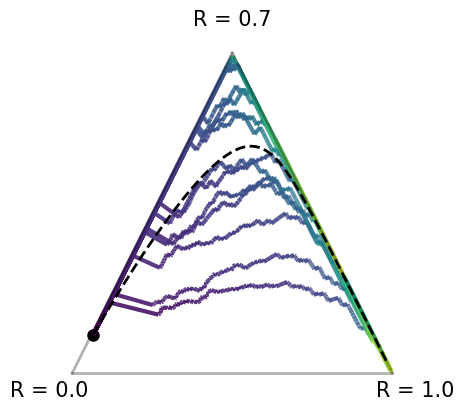
\includegraphics[width=\textwidth]{articles/baselines/figs/reproduced_simplex_npg/natural_value_00.png}
    \caption{$b_\theta=V^{\pi_\theta}$}
    \label{fig:v}
  \end{subfigure}
  \caption{ \label{fig:trajectories}  We plot 15 different trajectories of natural policy gradient with softmax parameterization, when using various baselines, on a 3-arm bandit problem with rewards $(1,0.7,0)$ and stepsize $\alpha = 0.025$ and $\theta_0 = (0, 3, 5)$. The black dot is the initial policy and colors represent time, from purple to yellow. The dashed black line is the trajectory when following the true gradient (which is unaffected by the baseline). Different values of $\epsilon$ denote different perturbations to the minimum-variance baseline. We see some cases of convergence to a suboptimal policy for both $\epsilon = -\nicefrac{1}{2}$ and $\epsilon = 0$. This does not happen for the larger baseline $\epsilon = \nicefrac{1}{2}$ or the value function as baseline. Figure made with Ternary~\citep{pythonternary}.}
\end{figure*}



\section{Baselines, learning dynamics \& exploration}
\label{sec:committal}

The problem defined in Eq.~\ref{eq:bandit_loss} can be solved by gradient ascent. Given access only to samples, the true gradient cannot generally be computed and the true update is replaced with a stochastic one, resulting in the following update:
\begin{align}
    \theta_{t+1} &= \theta_t + \frac{\alpha}{N} \sum_i r(a_i) \nabla_\theta \log \pi_\theta(a_i) \label{eq:mc_update} \; ,
\end{align}
where $a_i$ are actions drawn according to the agent's current policy $\pi_\theta$, $\alpha$ is the stepsize, and $N$, which can be 1, is the number of samples used to compute the update.
To reduce the variance of this estimate without introducing bias, we can introduce a baseline $b$, resulting in the gradient estimate $(r(a_i) - b) \nabla_\theta \log \pi_\theta(a_i)$.


While the choice of baseline is known to affect the variance, we show that baselines can also lead to qualitatively different behaviour of the optimization process, even when the variance is the same. This difference cannot be explained by the expectation or variance, quantities which govern the usual bounds for convergence rates~\citep{bottou2018optimization}. 


\subsection{Committal and non-committal behaviours}

To provide a complete picture of the optimization process, we analyze the evolution of the policy during optimization.
We start in a simple setting, a deterministic three-armed bandit, where it is easier to produce informative visualizations. 

To eliminate variance as a potential confounding factor, we consider different baselines with the same variance. We start by computing the baseline leading to the minimum-variance of the gradients for the algorithm we use. For vanilla policy gradient, we have $b^*_\theta = \frac{\E[r(a_i) \|\nabla \log \pi_\theta (a_i)\|^2_2 ] }{\E[ \|\nabla \log \pi_\theta (a_i) \|^2_2] } $ ~\citep{peters2008reinforcement, greensmith2004variance} (see Appendix~\ref{app:optimal_baseline} for details and the NPG version). Note that this baseline depends on the current policy and changes throughout the optimization. As the variance is a quadratic function of the baseline, the two baselines $b^+_\theta = b^*_\theta + \epsilon$ and $b^-_\theta = b^*_\theta - \epsilon$ result in gradients with the same variance (see Appendix \ref{app:var_perturbed_baseline} for details). Thus, we use these two perturbed baselines to demonstrate that there are phenomena in the optimization process that variance~cannot~explain.

Fig.~\ref{fig:trajectories} presents fifteen learning curves on the probability simplex representing the space of possible policies for the three-arm bandit, when using NPG and a softmax parameterization. We choose $\epsilon = \nicefrac{1}{2}$ to obtain two baselines with the same variance: $b^+_\theta = b^*_\theta + \nicefrac{1}{2}$ and $b^-_\theta = b^*_\theta - \nicefrac{1}{2}$.

Inspecting the plots, the learning curves for $\epsilon = -\nicefrac{1}{2}$ and $\epsilon = \nicefrac{1}{2}$ are qualitatively different, even though the gradient estimates have the same variance. For $\epsilon = -\nicefrac{1}{2}$, the policies quickly reach a deterministic policy (i.e., a neighborhood of a corner of the probability simplex), which can be suboptimal, as indicated by the curves ending up at the policy choosing action 2. On the other hand, for $\epsilon=\nicefrac{1}{2}$, every learning curve ends up at the optimal policy, although the convergence might be slower. The learning curves also do not deviate much from the curve for the true gradient. 
Again, these differences cannot be explained by the variance since the baselines result in identical variances. 


Additionally, for $b_\theta=b^*_\theta$, the learning curves spread out further. Compared to $\epsilon=\nicefrac{1}{2}$, some get closer to the top corner of the simplex, leading to convergence to a suboptimal solution, suggesting that the minimum-variance baseline may be worse than other, larger baselines. In the next section, we theoretically substantiate this and show that, for NPG, it is possible to converge to a suboptimal policy with the minimum-variance baseline; but there are larger baselines that guarantee convergence to an optimal~policy.

We look at the update rules to explain these different behaviours. When using a baseline $b$ with NPG, sampling $a_i$ results in the update
\begin{align*}
    \theta_{t+1} &= \theta_t + \alpha  [r(a_i)-b] F_\theta^{-1} \nabla_\theta \log \pi_\theta(a_i) \label{eq:npg_bandit_update} \\
    &= \theta_t + \alpha \frac{r(a_i)-b}{\pi_\theta(a_i)} \mathbf{1}_{a_i} + \alpha\lambda e
\end{align*}
where $F_\theta^{-1} = \E_{a \sim \pi} [\nabla \log \pi_\theta (a) \nabla \log \pi_\theta (a)^\top]$, $\mathbf{1}_{a_i}$ is a one-hot vector with $1$ at index $i$, and $\lambda e$ is a vector containing $\lambda$ in each entry.  The second line follows for the softmax policy (see Appendix \ref{app:npg_softmax_bandit}) and $\lambda$ is arbitrary since shifting $\theta$ by a constant does not change the policy.


Thus, supposing we sample action $a_i$, if $r(a_i) - b$ is positive, which happens more often when the baseline $b$ is small (more negative), the update rule will increase the probability $\pi_\theta(a_i)$. This leads to an increase in the probability of taking the actions the agent took before, regardless of their quality (see Fig.\ref{fig:-1} for $\epsilon=-\nicefrac{1}{2}$). Because the agent is likely to choose the same actions again, we call this \textit{committal} behaviour.

While a smaller baseline leads to committal behaviour, a larger (more positive) baseline makes the agent second-guess itself. If $r(a_i) - b$ is negative, which happens more often when $b$ is large, the parameter update decreases the probability $\pi_\theta(a_i)$ of the sampled action $a_i$, reducing the probability the agent will re-take the actions it just took, while increasing the probability of other actions. This might slow down convergence but it also makes it harder for the agent to get stuck. This is reflected in the $\epsilon = \nicefrac{1}{2}$ case (Fig.\ref{fig:1}), as all the learning curves end up at the optimal policy. We call this \textit{non-committal} behaviour.

While the previous experiments used perturbed variants of the minimum-variance baseline to control for the variance, this baseline would usually be infeasible to compute in more complex MDPs. Instead, a more typical choice of baseline would be the value function~\citep[Ch.~13]{sutton18book}, which we evaluate in Fig. \ref{fig:v}.
Choosing the value function as a baseline generated trajectories converging to the optimal policy, even though their convergence may be slow, despite it not being the minimum variance baseline.
The reason becomes clearer when we write the value function as $\displaystyle V^\pi = b^\ast_\theta - \tfrac{\textrm{Cov}(r, \|\nabla \log \pi\|^2)}{\E[\|\nabla \log \pi\|^2]}$ (see Appendix \ref{app:value_minvar_baseline}). The term $\textrm{Cov}(r, \|\nabla \log \pi\|^2)$ typically becomes negative as the gradient becomes smaller on actions with high rewards during the optimization process, leading to the value function being a noncommittal baseline, justifying a choice often made by practitioners. 

Additional empirical results can be found in Appendix \ref{app:exp_3armbandit} for natural policy gradient and vanilla policy gradient for the softmax parameterization. Furthermore, we explore the use of different parameterizations: First, we test projected stochastic gradient ascent and directly optimizing the policy probabilities $\pi_\theta(a)$. Next, we try the escort transform \citep{mei2020escaping}, which was designed to improve the curvature of the objective. We find qualitatively similar results in all cases; baselines can induce \textit{committal} and \textit{non-committal} behaviour. 

\section{Convergence to suboptimal policies with natural policy gradient (NPG)}

We empirically showed that PG algorithms can reach suboptimal policies and that the choice of baseline can affect the likelihood of this occurring. 
In this section, we provide theoretical results proving that it is indeed possible to converge to a suboptimal policy when using NPG. 
We discuss how this finding fits with existing convergence results and why standard assumptions are not satisfied in this setting. 

\subsection{A simple example}\label{sec:divergence_example}

Standard convergence results assume access to the true gradient~\citep[e.g.,][]{agarwal2019optimality} or, in the stochastic case, assume that the variance of the updates is uniformly bounded for all parameter values~\citep[e.g.,][]{bottou2018optimization}.
These assumptions are in fact quite strong and are violated in a simple two-arm bandit problem with fixed rewards. 
Pulling the optimal arm gives a reward of $r_1 = +1$, while pulling the suboptimal arm leads to a reward of $r_0 = 0$. We use the sigmoid parameterization and call $p_t = \sigma(\theta_t)$ the probability of sampling the optimal arm at time $t$.

Our stochastic estimator of the natural gradient is %
\begin{align*}
g_t = \left\{
                \begin{array}{l}
                  \frac{1 - b}{p_t}, \text{with probability}\ p_t \\
                  \frac{b}{1-p_t}, \text{with probability}\ 1-p_t,
                \end{array}
              \right.
\end{align*}
where $b$ is a baseline that does not depend on the action sampled at time $t$ but may depend on $\theta_t$. 
By computing the variance of the updates, $\textrm{Var}[g_t] =   \tfrac{(1-p_t - b)^2}{p_t (1-p_t)}$, we notice it is unbounded when the policy becomes deterministic, i.e. $p_t \to 0$ or $p_t \to 1$, violating the assumption of uniformly bounded variance, unless $b = 1-p_t$, which is the optimal baseline.
Note that using vanilla (non-natural) PG would, on the contrary, yield a bounded variance. In fact, we prove a convergence result in its favour in Appendix \ref{app:theory_2arm} (Prop. \ref{prop_vpg_cv}).

For NPG, the proposition below establishes potential convergence to a suboptimal arm and we demonstrate this~empirically~in~Fig.~\ref{fig:divergence_2arm_bandit}.

\begin{restatable}[]{proposition}{divtwoarms}
Consider a two-arm bandit with rewards $1$ and $0$ for the optimal and suboptimal arms, respectively. Suppose we use natural policy gradient starting from $\theta_0$, with a fixed baseline $b < 0$, and fixed stepsize $\alpha > 0$. If the policy samples the optimal action with probability $\sigma(\theta)$, then the probability of picking the suboptimal action forever and having $\theta_t$ go to $-\infty$ is strictly positive.
Additionally, if $\theta_0 \le 0$, we have
\[ P(\textup{suboptimal action forever}) \ge (1-e^{\theta_0}) (1-e^{\theta_0 + \alpha b})^{-\frac{1}{\alpha b}}. \]
\label{proposition_divergence}
\end{restatable}
\vspace{-0.8cm}
\begin{proof}
All the proofs may be found in the appendix.
\end{proof}

\begin{figure}[t!]
\centering
\begin{subfigure}[b]{0.32\linewidth}   
    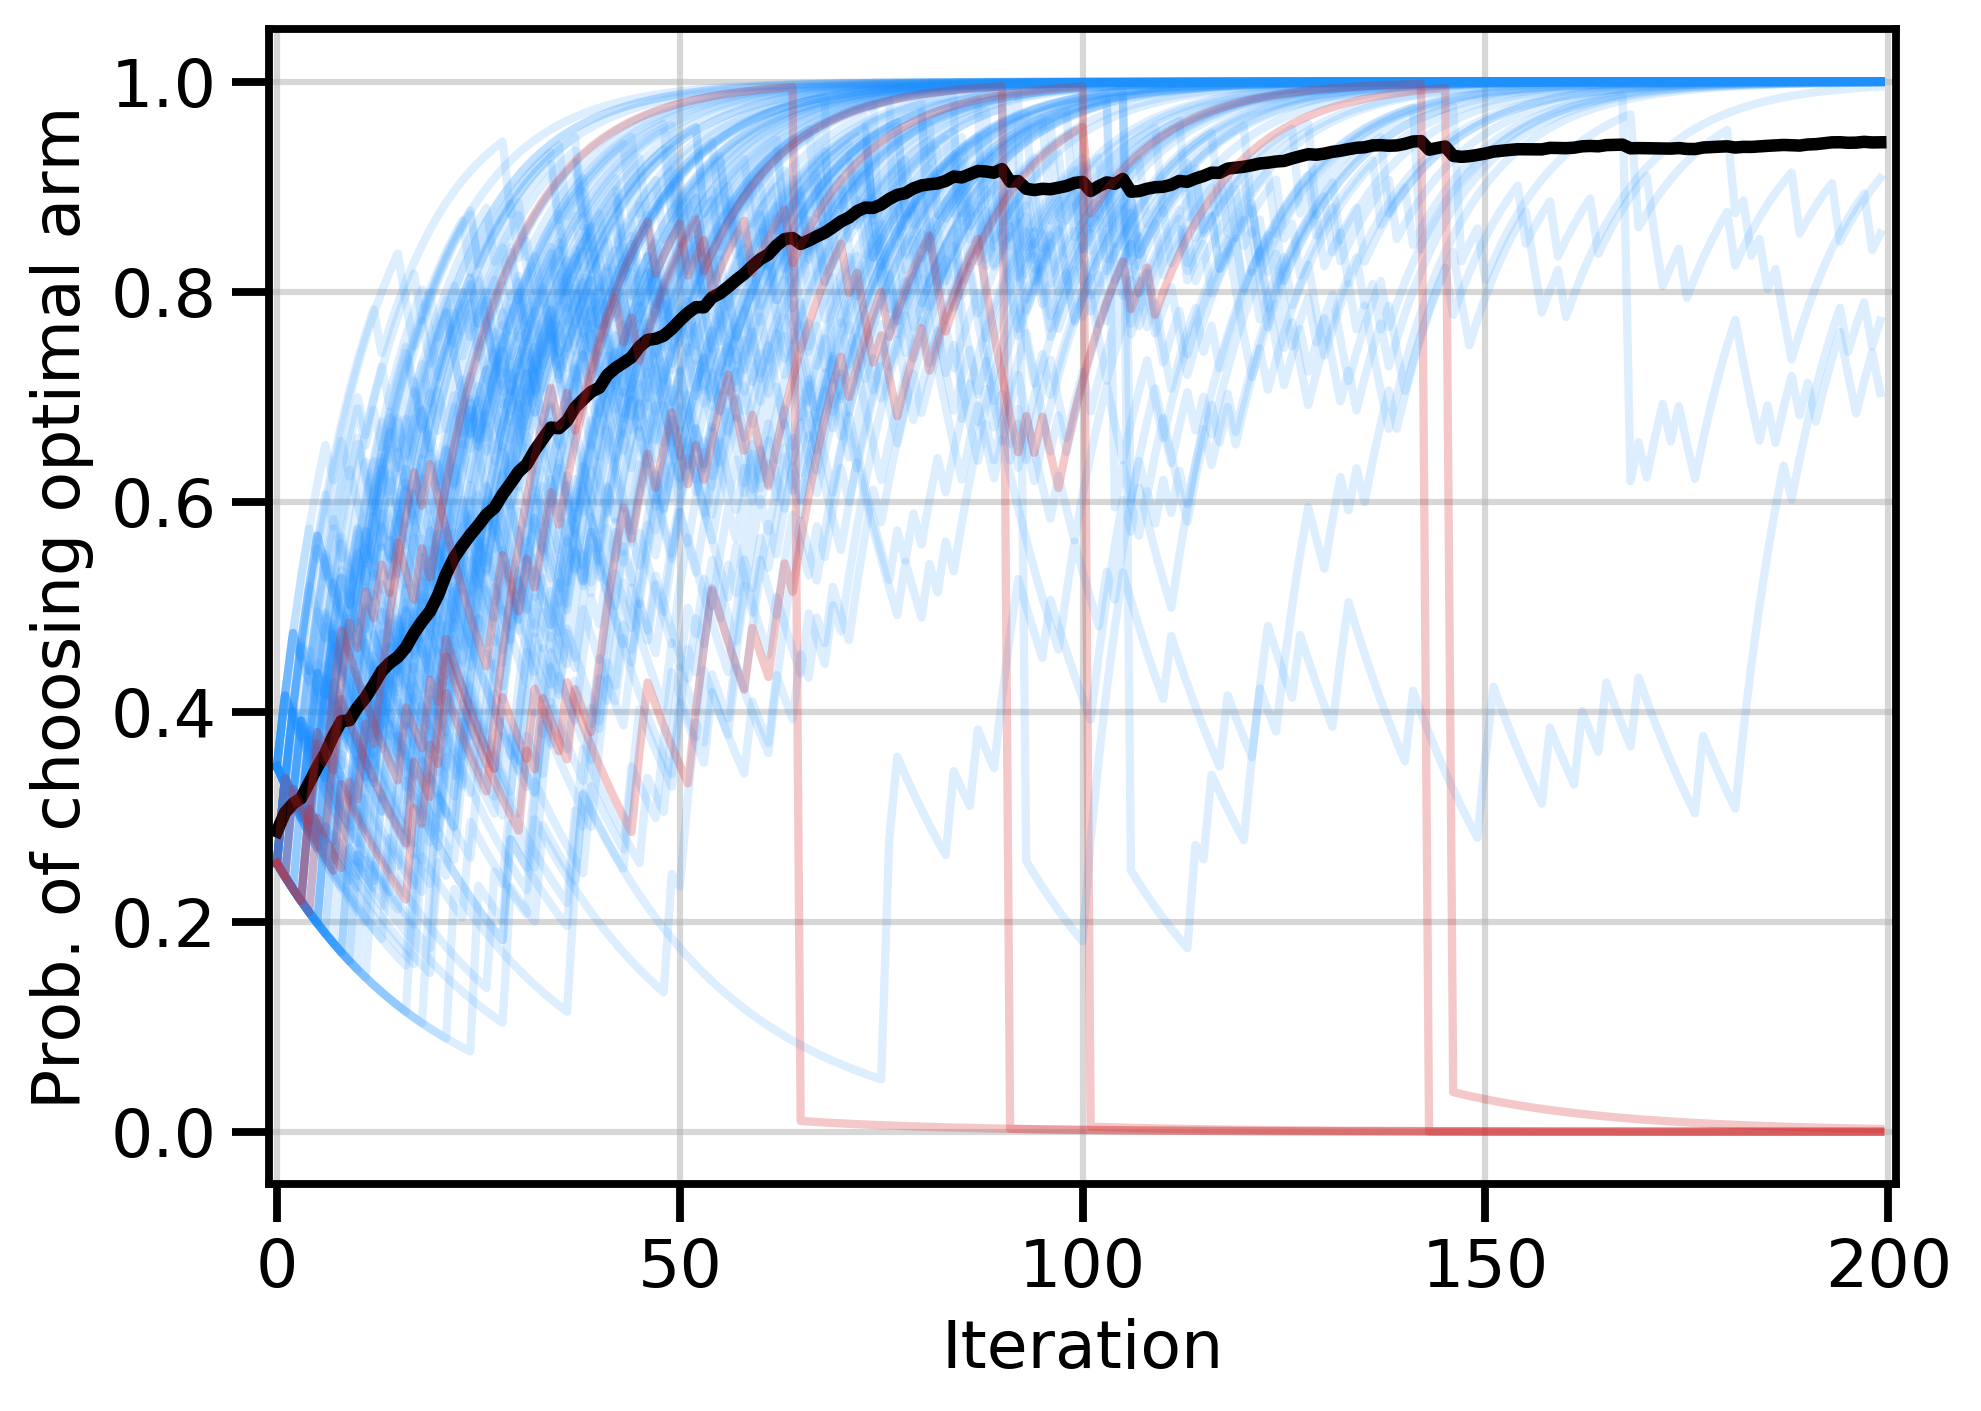
\includegraphics[width=\textwidth]{articles/baselines/figs/paper/bandit_committal_005.png}
    \caption{$\alpha=0.05$}
\end{subfigure}
\begin{subfigure}[b]{0.32\linewidth}   
    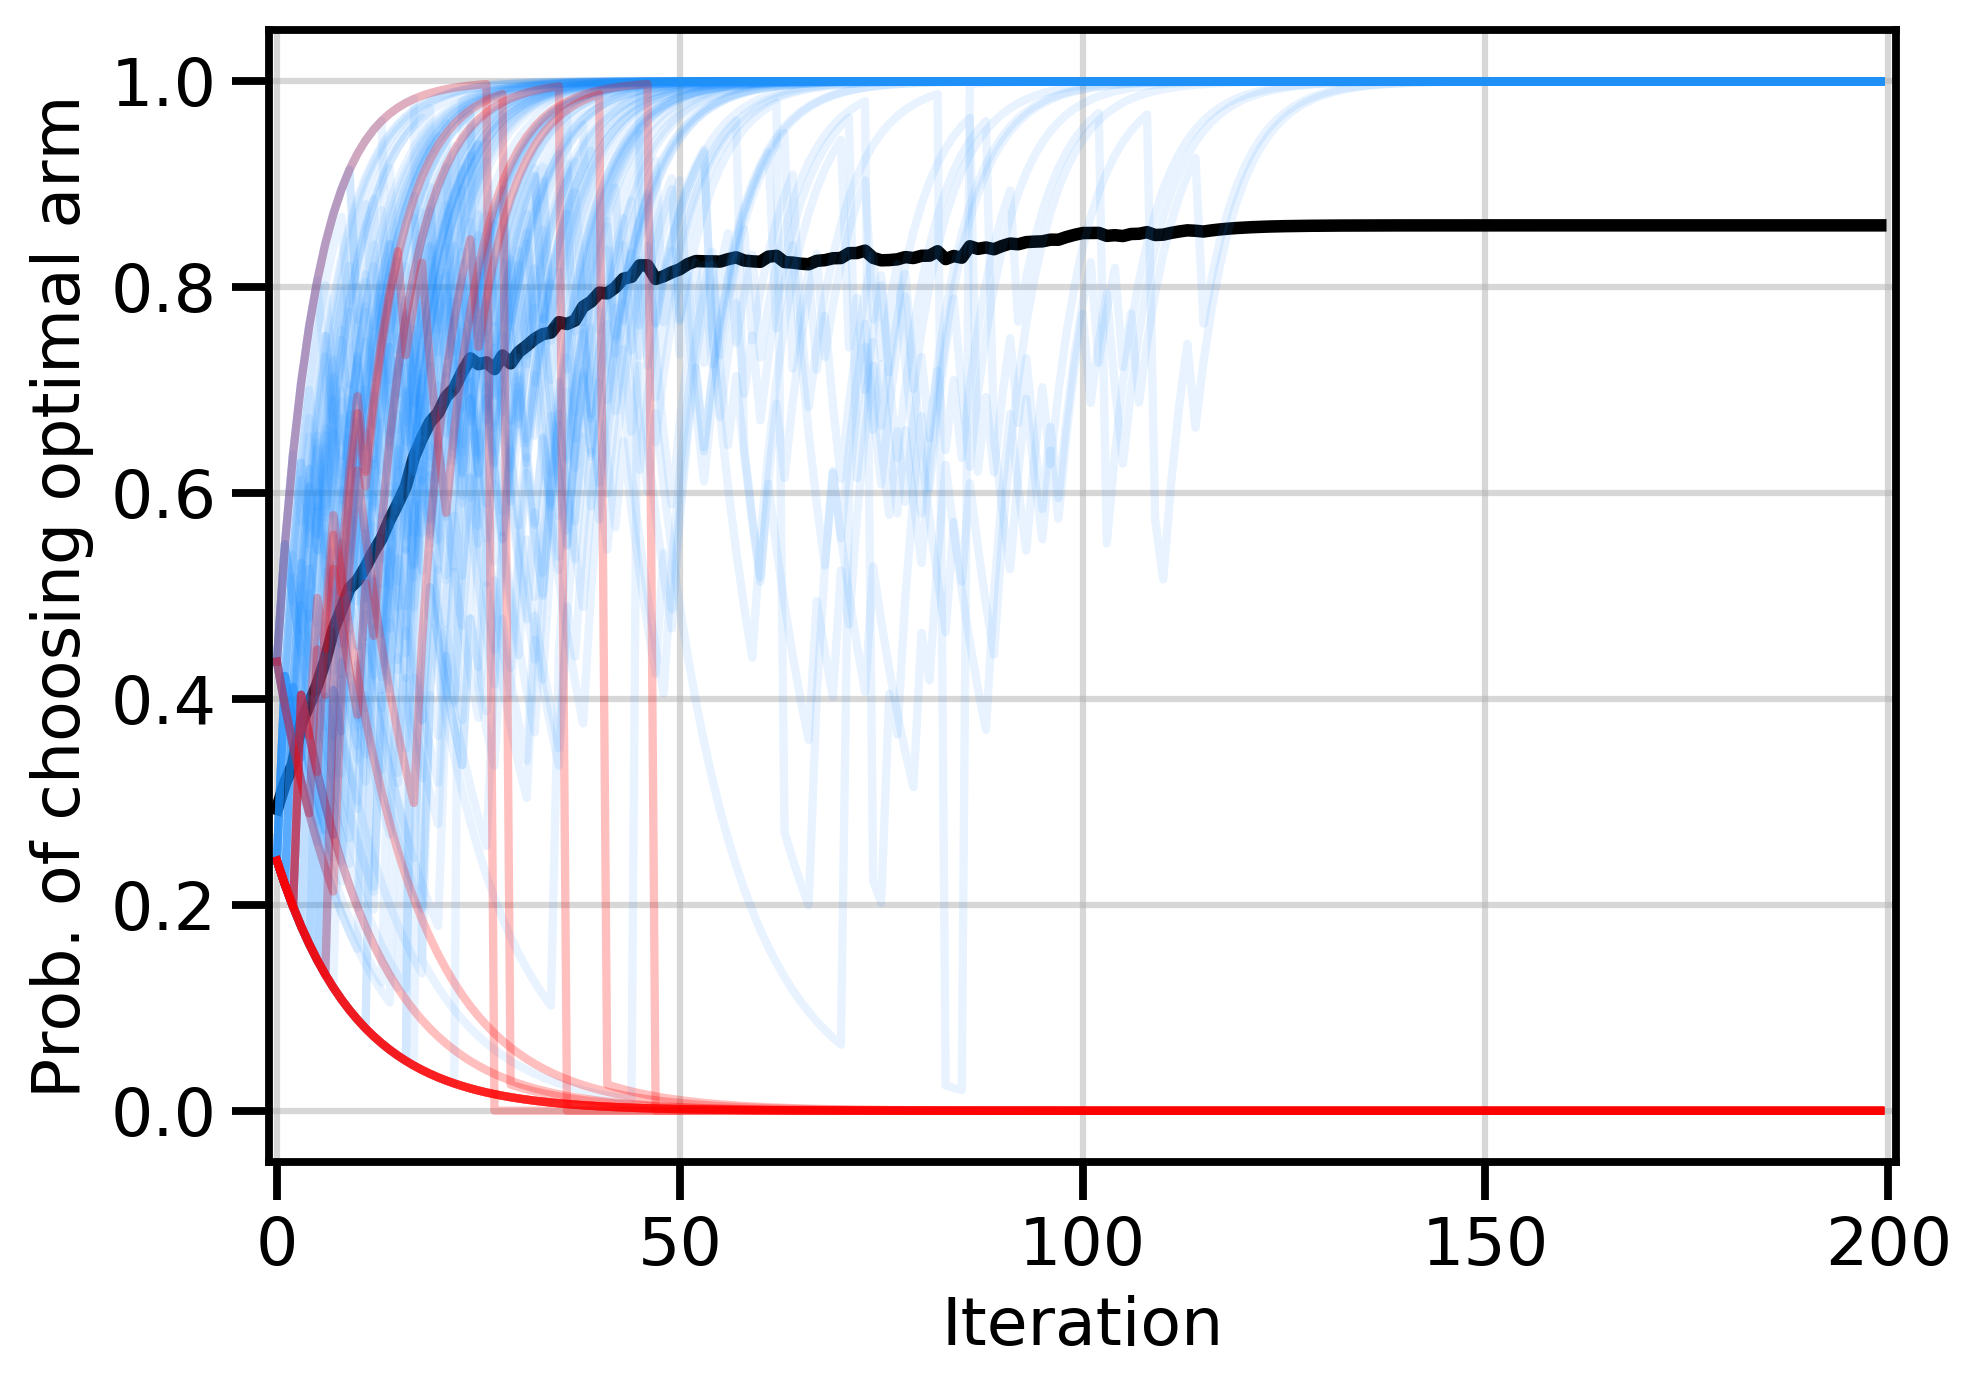
\includegraphics[width=\textwidth]{articles/baselines/figs/paper/bandit_committal.png}
    \caption{$\alpha=0.1$}
\end{subfigure}
\begin{subfigure}[b]{0.32\linewidth}   
    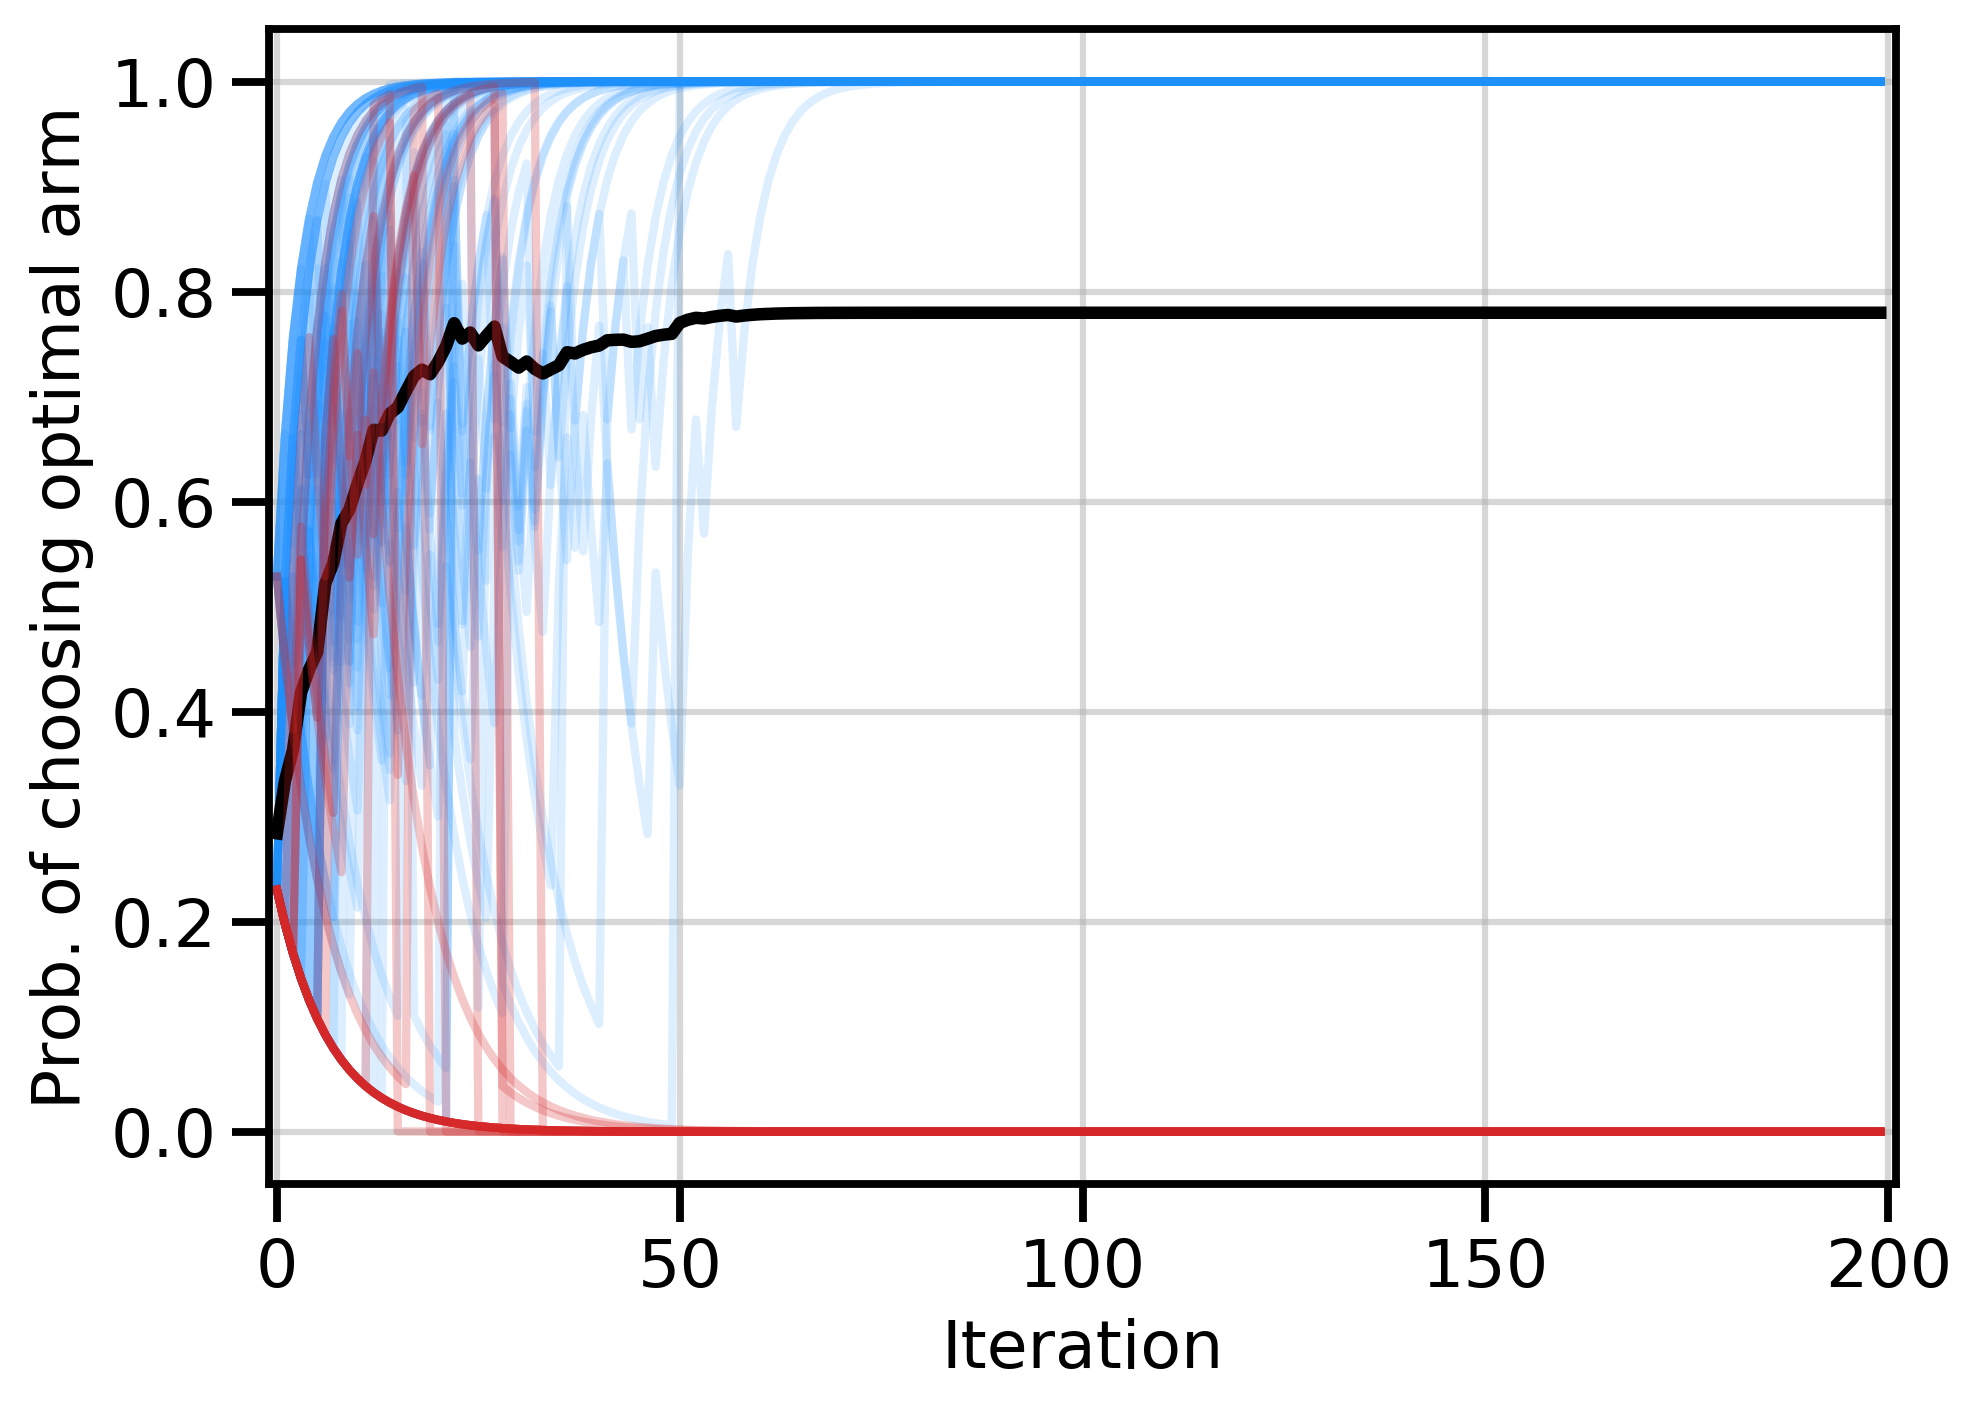
\includegraphics[width=\textwidth]{articles/baselines/figs/paper/bandit_committal_015.png}
    \caption{$\alpha=0.15$}
\end{subfigure}

\caption{Learning curves for 100 runs of 200 steps, on the two-arm bandit, with baseline $b\!=\!-1$ for three different stepsizes $\alpha$. \emph{Blue:} Curves converging to the optimal policy. \emph{Red:} Curves  converging to a suboptimal policy. \emph{Black:} Avg. performance. 
The number of runs that converged to the suboptimal solution are 5\%, 14\% and 22\% for the three $\alpha$'s. Larger $\alpha$'s are more prone to getting stuck at a suboptimal solution but settle on a deterministic policy more quickly.}
\label{fig:divergence_2arm_bandit}
\end{figure}

The updates provide some intuition as to why there is convergence to suboptimal policies. The issue is the \textit{committal} nature of the baseline. Choosing an action leads to an increase of that action's probability, even if it is a poor choice. Choosing the suboptimal arm leads to a decrease in $\theta$ by $\tfrac{\alpha b}{1-p_t}$, thus increasing the probability the same arm is drawn again and further decreasing $\theta$. By checking the probability of this occurring forever, $P(\text{suboptimal arm forever}) = \prod_{t=1}^\infty (1-p_t)$, we show that $1-p_t$ converges quickly enough to 1 that the infinite product is nonzero, showing it is possible to get trapped choosing the wrong arm forever~(Prop. \ref{proposition_divergence}), and $\theta_t \to -\infty$ as $t$ grows.

This issue could be solved by picking a baseline with lower variance. For instance, the minimum-variance baseline $b = 1 - p_t$ leads to $0$ variance and both possible updates are equal to $+\alpha$, guaranteeing that $\theta \to +\infty$, thus convergence. In fact, any baseline $b \in (0,1)$ suffices since both updates are positive and greater than $\alpha \min(b, 1-b)$. However, this is not always the case, as we show in the next section.

To decouple the impact of the variance with that of the committal nature of the baseline, Prop.~\ref{prop:2armed-perturbedminvar} analyzes the learning dynamics in the two-arm bandit case for perturbations of the optimal baseline, i.e. we study baselines of the form $b = b^* + \epsilon$ and show how $\epsilon$, and particularly its sign, affects learning. Note that, because the variance is a quadratic function with its minimum in $b^*$, both $+\epsilon$ and $-\epsilon$ have the same variance. Our findings can be summarized as follows:
\begin{proposition}
    \label{prop:2armed-perturbedminvar}
    For the two-armed bandit defined in Prop.~\ref{proposition_divergence}, when using a perturbed min-variance baseline $b = b^* + \epsilon$, the value of $\epsilon$ determines the learning dynamics as follows:
    \begin{itemize}%
        \item For $\epsilon < -1$, there is a positive probability of converging to the suboptimal arm.
        \item For $\epsilon \in (-1, 1)$, we have convergence in probability to the optimal policy.
        \item For $\epsilon \ge 1$, the supremum of the iterates goes to $+\infty$ in probability.
    \end{itemize}
\end{proposition}


While the proofs can be found in Appendix~\ref{sec:appendix_perturbed_minvar}, we provide here some intuition behind these results.

For $\epsilon < -1$, we reuse the same argument as for $b<0$ in Prop.~\ref{proposition_divergence}. The probability of drawing the correct arm can decrease quickly enough to lead to convergence to the suboptimal arm.

For $\epsilon \in (-1,1)$, the probability of drawing the correct arm cannot decrease too fast. Hence, although the updates, as well as the variance of the gradient estimate, are potentially unbounded, we still have convergence to the optimal solution in probability.

Finally, for $\eps \ge 1$, we can reuse an intermediate argument from the $\epsilon \in (0,1)$ case to argue that for any threshold $C$, the parameter will eventually exceed that threshold. For $\epsilon \in (0,1)$, once a certain threshold is crossed, the policy is guaranteed to improve at each step. However, with a large positive perturbation, updates are larger and we lose this additional guarantee, leading to the weaker result.

We want to emphasize that not only we get provably different dynamics for $\epsilon < -1$ and $\eps \ge 1$, showing the importance of the sign of the perturbation, but that there also is a sharp transition around $|\epsilon| = 1$, which cannot be captured solely by the variance.

The above analysis was specific to these updates. To predict committal vs. non-committal behaviour more generally, it may be possible to utilize higher order moments or other distributional properties, even when the mean and variance is the same.
Unfortunately, it is difficult to utilize higher-moment information in theoretical bounds in a general manner as Markov-type inequalities do not take into account the sign of the higher moment, which we think is where the committal vs. non-committal distinction would appear.




\subsection{Reducing variance with baselines can be detrimental}
\label{sec:reducing_detrimental}
As we saw with the two-armed bandit, the direction of the updates is important in assessing convergence. More specifically, problems can arise when the choice of baseline induces committal behaviour.
We now show a different bandit setting where committal behaviour happens even when using the minimum-variance baseline, thus leading to convergence to a suboptimal policy. Furthermore, we design a better baseline which ensures all updates move the parameters towards the optimal policy. This cements the idea that the quality of parameter updates must not be analyzed in terms of variance but rather in terms of the probability of going in a bad direction, since a baseline that induces higher variance leads to convergence while the minimum-variance baseline does not.
The following theorem summarizes this.

\begin{restatable}[]{theorem}{threearmedbandit}
There exists a three-arm bandit where using the stochastic natural gradient on a softmax-parameterized policy with the minimum-variance baseline can lead to convergence to a suboptimal policy with probability $\rho > 0$, and there is a different baseline (with larger variance) which results in convergence to the optimal policy with probability~1.
\label{proposition_threearmedbandit}
\end{restatable}
The bandit used in this theorem is the one we used for the experiments depicted in Fig.~\ref{fig:trajectories}.
The key is that the minimum-variance baseline can be lower than the second best reward; so pulling the second arm will increase its probability and induce committal behaviour.
This can cause the agent to prematurely commit to the second arm and converge to the wrong policy.
On the other hand, using any baseline whose value is between the optimal reward and the second best reward, which we term a \textit{gap} baseline, will always increase the probability of the optimal action at every step, no matter which arm is drawn. Since the updates are sufficiently large at every step, this is enough to ensure convergence with probability 1, despite the higher variance compared to the minimum variance baseline.
The key is that whether a baseline underestimates or overestimates the second best reward can affect the algorithm convergence and this is more critical than the resulting variance of the gradient estimates.


As such, more than lower variance, good baselines are those that can assign positive effective returns to the good trajectories and negative effective returns to the others. These results cast doubt on whether finding baselines which minimize variance is a meaningful goal to pursue. The baseline can affect optimization in subtle ways, beyond variance, and further study is needed to identify the true causes of some improved empirical results observed in previous works. This importance of the sign of the returns, rather than their exact value, echoes with the cross-entropy method~\citep{de2005tutorial}, which maximizes the probability of the trajectories with the largest returns, regardless of their actual value.


\section{Off-policy sampling} 

So far, we have seen that \textit{committal} behaviour can be problematic as it can cause convergence to a suboptimal policy. This can be especially problematic when the agent follows a near-deterministic policy as it is unlikely to receive different samples which would move the policy away from the closest deterministic one, regardless of the quality of that policy.

Up to this point, we assumed that actions were sampled according to the current policy, a setting known as \emph{on-policy}. This setting couples the updates and the policy and is a root cause of the \textit{committal} behaviour: the update at the current step changes the policy, which affects the distribution of rewards obtained and hence the next updates. 
However, we know from the optimization literature that bounding the variance of the updates will lead to convergence \citep{bottou2018optimization}. As the variance becomes unbounded when the probability of drawing some actions goes to 0, a natural solution to avoid these issues is to sample actions from a behaviour policy that selects every action with sufficiently high probability.
Such a policy would make it impossible to choose the same, suboptimal action forever. 

\subsection{Convergence guarantees with IS}

Because the behaviour policy changed, we introduce importance sampling (IS) corrections to preserve the unbiased updates~\citep{kahn1951estimation, precup2000eligibility}. 
These changes are sufficient to guarantee convergence for any baseline:

\begin{restatable}[]{proposition}{is}
\label{lem:main_off-policy_IS}
Consider a $n$-armed bandit with stochastic rewards with bounded support and a unique optimal action. The behaviour policy $\mu_t$ selects action $i$ with probability $\mu_t(i)$ and let $\epsilon_t = \min_i \mu_t(i)$. When using NPG with importance sampling and a bounded baseline $b$, if $\lim_{t \to \infty} t \ \epsilon_t^2 = +\infty$ , then the target policy $\pi_t$ converges to the optimal policy in probability.
\end{restatable}
\begin{proof} 
\textit{(Sketch)}
Using Azuma-Hoeffding's inequality, we can show that for well chosen constants $\Delta_i, \delta$ and $C > 0$ ,
\begin{eqnarray*}
\sP\left( \theta_t^1 \ge  \theta_0^1 + \alpha \delta \Delta_1 t\right) %
&\ge& 1- \exp \left( -\frac{\delta^2 \Delta_1^2}{2 C^2}t \epsilon_t^2 \right)\\
\end{eqnarray*} 
where $\theta^1$ is the parameter associated to the optimal arm.
Thus if $\lim_{t\to\infty} t \epsilon_t^2 = +\infty$, the RHS goes to $1$. 
In a similar manner, we can upper bound $\sP\left( \theta_t^i \ge  \theta_0^i + \alpha \delta \Delta_i t\right)$ for all suboptimal arms, and 
applying an union bound, we get the desired result.
\end{proof}
\vspace{-3mm}

The condition on $\mu_t$ imposes a cap on how fast the behaviour policy can become deterministic: no faster than $t^{-1/2}$. Intuitively, this ensures each action is sampled sufficiently often and prevents premature convergence to a suboptimal policy.
The condition is satisfied for any sequence of behaviour policies which assign at least $\epsilon_t$ probability to each action at each step, such as $\epsilon$-greedy policies. It also holds if $\epsilon_t$ decreases over time at a sufficiently slow rate. By choosing as behaviour policy $\mu$ a linear interpolation between $\pi$ and the uniform policy, $\mu(a) = (1-\gamma) \pi(a) + \frac{\gamma}{K}, \gamma \in (0,1]$, where $K$ is the number of arms, we recover the classic EXP3 algorithm~\citep{auer2002nonstochastic, seldin2012evaluation}.

We can also confirm that this condition is not satisfied for the simple example we presented when discussing convergence to suboptimal policies. There, $p_t$ could decrease exponentially fast since the tails of the sigmoid function decay exponentially and the parameters move by at least a constant at every step. In this case, $\epsilon_t = \Omega (e^{-t})$, resulting in $\lim_{t\to \infty} t e^{-2 t} = 0$, so Proposition~\ref{lem:main_off-policy_IS} does not apply.

\subsection{Importance sampling, baselines \& variance}
As we have seen, using a separate behaviour policy that samples all actions sufficiently often may lead to stronger convergence guarantees, even if it increases the variance of the gradient estimates in most of the space, as what matters is what happens in the high variance regions, which are usually close to the boundaries. Fig.~\ref{fig:simplex_variance} shows the ratios of gradient variances between on-policy PG without baseline, on-policy PG with the minimum variance baseline, and off-policy PG using importance sampling~(IS) where the sampling distribution is $\mu(a) = \frac{1}{2} \pi(a) + \frac{1}{6}$, i.e. a mixture of the current policy $\pi$ and the uniform distribution. While using the minimum variance baseline decreases the variance on the entire space compared to not using a baseline, IS actually \emph{increases} the variance when the current policy is close to uniform. However, IS does a much better job at reducing the variance close to the boundaries of the simplex, where it actually matters to guarantee convergence.

\begin{figure}[t!]
\begin{center}
    \begin{subfigure}[b]{0.08\linewidth}
    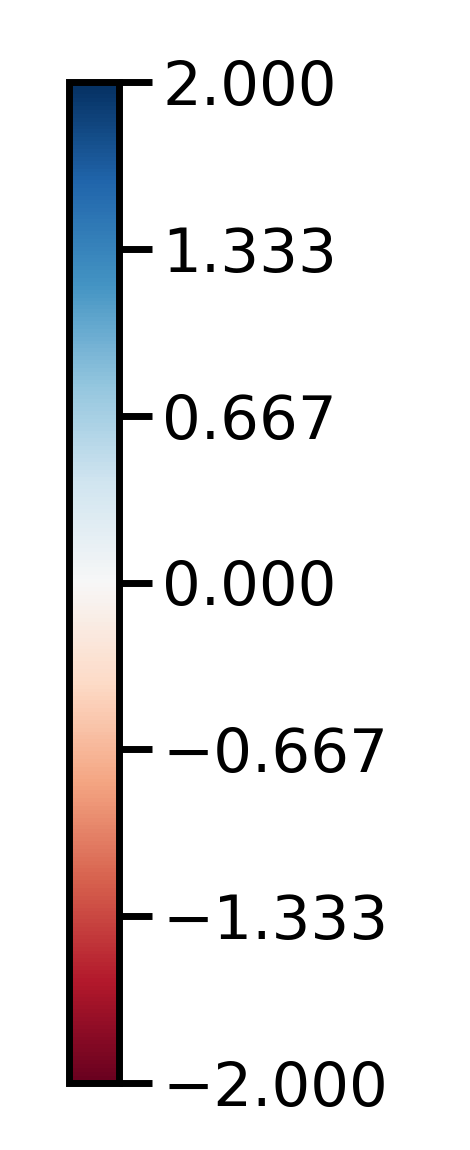
\includegraphics[trim={2cm 1.5cm 2cm 0},clip,width=\textwidth]{articles/baselines/figs/simplex_plots/colorbar_vertical.png}
    \label{fig:is_baseline}
  \end{subfigure}
  \begin{subfigure}[b]{.27\linewidth}
    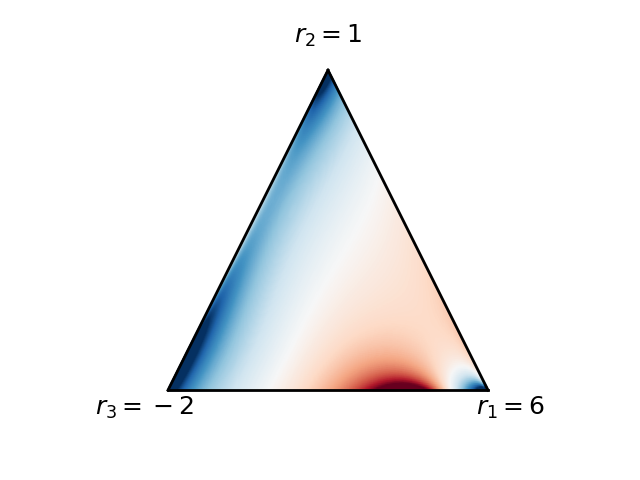
\includegraphics[trim={2cm 1.5cm 2cm 0mm},clip, width=\textwidth]{articles/baselines/figs/simplex_plots/v_vs_is.png}
    \caption{{\color{myred}$b=0$} / {\color{myblue}IS}.}
  \end{subfigure}
  \begin{subfigure}[b]{0.27\linewidth}
    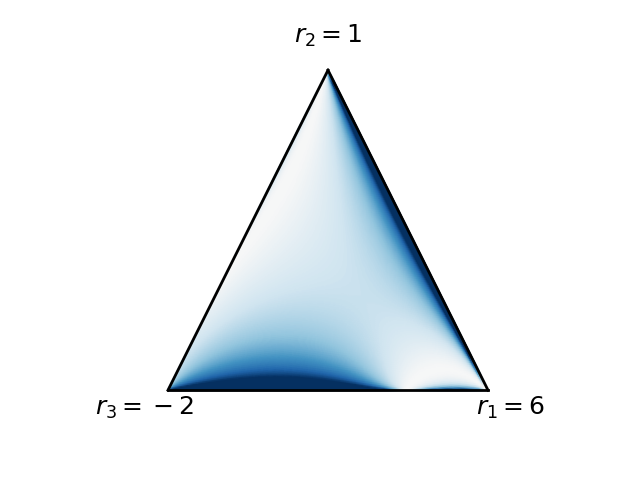
\includegraphics[trim={2cm 1.5cm 2cm 0},clip,width=\textwidth]{articles/baselines/figs/simplex_plots/v_vs_b.png}
    \caption{{\color{myred}$b=0$} / {\color{myblue}$b^\ast$}.}
  \end{subfigure}
  \begin{subfigure}[b]{0.27\linewidth}
    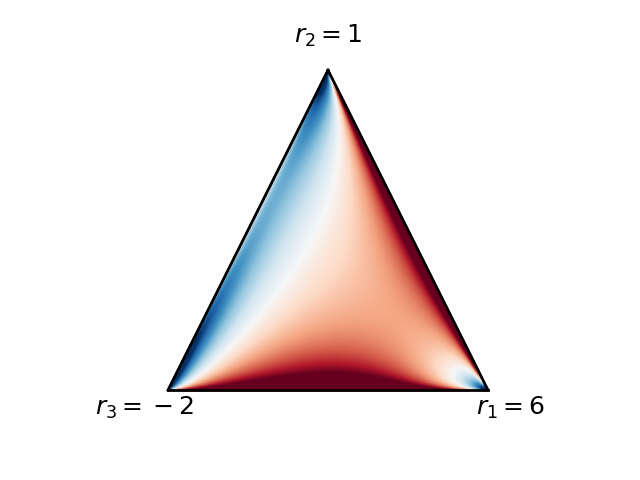
\includegraphics[trim={2cm 1.5cm 2cm 0},clip,width=\textwidth]{articles/baselines/figs/simplex_plots/b_vs_is.png}
    \caption{{\color{myred}$b^\ast$} / {\color{myblue}IS}.}
  \end{subfigure}
\caption{Comparison between the variance of different methods on a 3-arm bandit. Each plot depicts the $\log$ of the ratio between the variance of two approaches. For example, Fig. (a) depicts $\log \tfrac{\textrm{Var}[g_{b=0}]}{\textrm{Var}[g_{\text{IS}}]}$, the $\log$ of the ratio between the variance of the gradients of PG without a baseline and PG with IS. The triangle represents the probability simplex with each corner representing a deterministic policy on a specific arm. The method written in blue (resp. red) in each figure has lower variance in blue (resp. red) regions of the simplex. The sampling policy $\mu$, used in the PG method with IS, is a linear interpolation between $\pi$ and the uniform distribution, $\mu(a) = \frac{1}{2} \pi(a) + \frac{1}{6}$. Note that this is not the min. variance sampling distribution and it leads to higher variance than PG without a baseline in some parts of the simplex.} \label{fig:simplex_variance}
\end{center}
\end{figure}

This suggests that convergence of PG methods is not so much governed by the variance of the gradient estimates in general, but by the variance in the worst regions, usually near the boundary. While baselines can reduce the variance, they generally cannot prevent the variance in those regions from exploding, leading to the policy getting stuck. Thus, good baselines are not the ones reducing the variance across the space but rather those that can prevent the learning from reaching these regions altogether. Large values of $b$, such that $r(a_i) - b$ is negative for most actions, achieve precisely that. On the other hand, due to the increased flexibility of sampling distributions, IS can limit the nefariousness of these critical regions, offering better convergence guarantees despite not reducing variance~everywhere.

Importantly, although IS is usually used in RL to correct for the distribution of past samples~\citep[e.g.,][]{munos16retrace}, we advocate here for expanding the research on designing appropriate sampling distributions as done by~\citet{hanna2017data, hanna2018importance} and \citet{parmas2019unified}. This line of work has a long history in statistics~\citep[c.f.,][]{liu2008monte}. 

\subsection{Other mitigating strategies}
We conclude this section by discussing alternative strategies to mitigate the convergence issues. While they might be effective, and some are indeed used in practice, they are not without pitfalls.

First, one could consider reducing the stepsizes, with the hope that the policy would not converge as quickly towards a suboptimal deterministic policy and would eventually leave that bad region. Indeed, if we are to use vanilla PG in the two-arm bandit example, instead of NPG, this effectively reduces the stepsize by a factor of $\sigma(\theta)(1-\sigma(\theta))$ (the Fisher information). In this case, we are able to show convergence in probability to the optimal policy. See Proposition~\ref{prop_vpg_cv} in Appendix \ref{app:theory_2arm}.

Empirically, we find that, when using vanilla PG, the policy may still remain stuck near a suboptimal policy when using a negative baseline, similar to Fig.~\ref{fig:divergence_2arm_bandit}. While the previous proposition guarantees convergence eventually, the rate may be very slow, which remains problematic in practice. There is theoretical evidence that following even the true vanilla PG may result in slow convergence~\citep{schaul2019ray}, suggesting that the problem is not necessarily due to noise.

An alternative solution would be to add entropy regularization to the objective. By doing so, the policy would be prevented from getting too close to deterministic policies. While this might prevent convergence to a suboptimal policy, it would also exclude the possibility of fully converging to the optimal policy, though the policy may remain near it.

In bandits, EXP3 has been found not to enjoy high-probability guarantees on its regret so variants have been developed to address this deficiency \citep[c.f.][]{lattimore_szepesvari_2020}. For example, by introducing bias in the updates, their variance can be reduced significantly \cite{auer2002nonstochastic, neu2015explore}.
Finally, other works have also developed provably convergent policy gradient algorithms using different mechanisms, such as exploration bonuses or ensembles of policies~\citep{cai2019provably, efroni2020optimistic, agarwal2020pc}. 


\section{Extension to multi-step MDPs}
\begin{figure*}
\centering
 \begin{subfigure}[b]{0.21\linewidth}   
    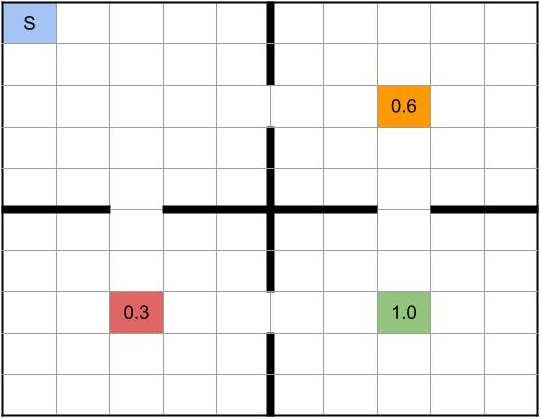
\includegraphics[trim={0cm -0.8cm 0cm 0},clip,width=\textwidth]{articles/baselines/figs/paper/Four_rooms.jpg}
    \caption{MDP}
    \label{fig:4rooms_mdp}
  \end{subfigure}
  \begin{subfigure}[b]{0.25\linewidth}
    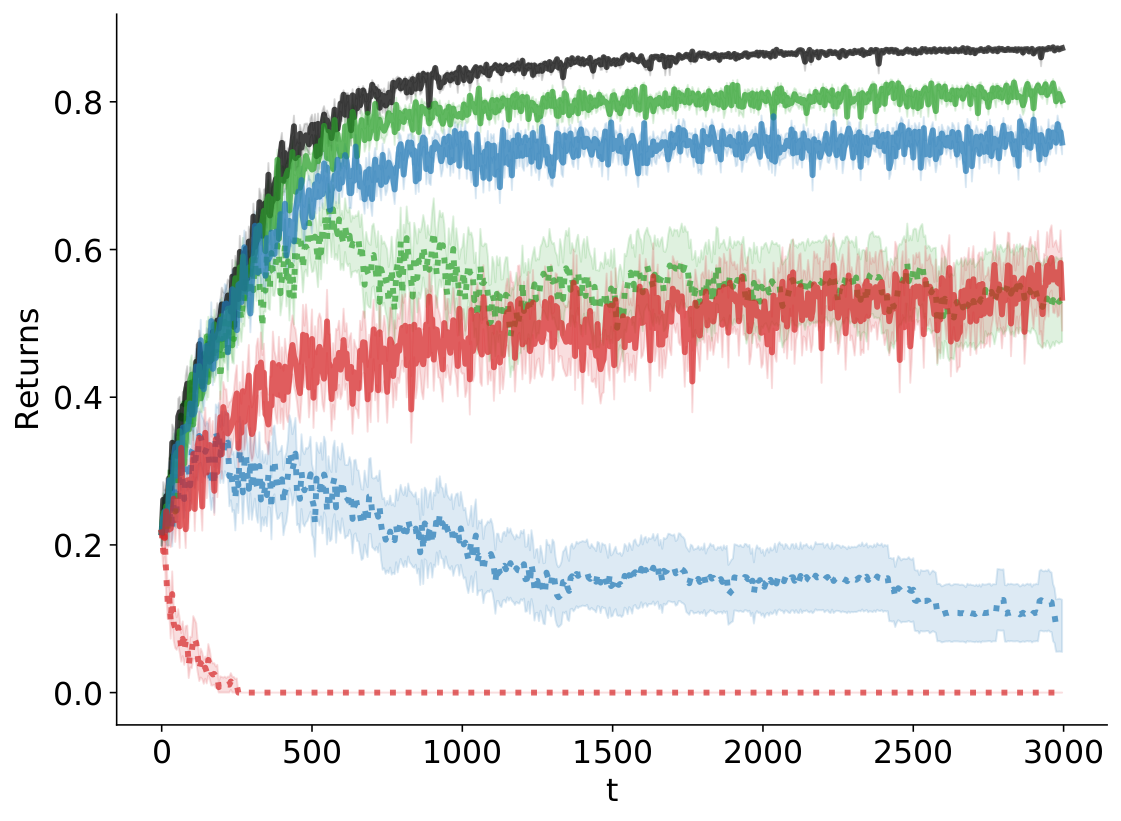
\includegraphics[width=\textwidth]{articles/baselines/figs/baseline_4rooms/NPG_returns.png}
    \caption{Returns}
    \label{fig:4rooms_return}
  \end{subfigure}
    \begin{subfigure}[b]{0.25\linewidth}
    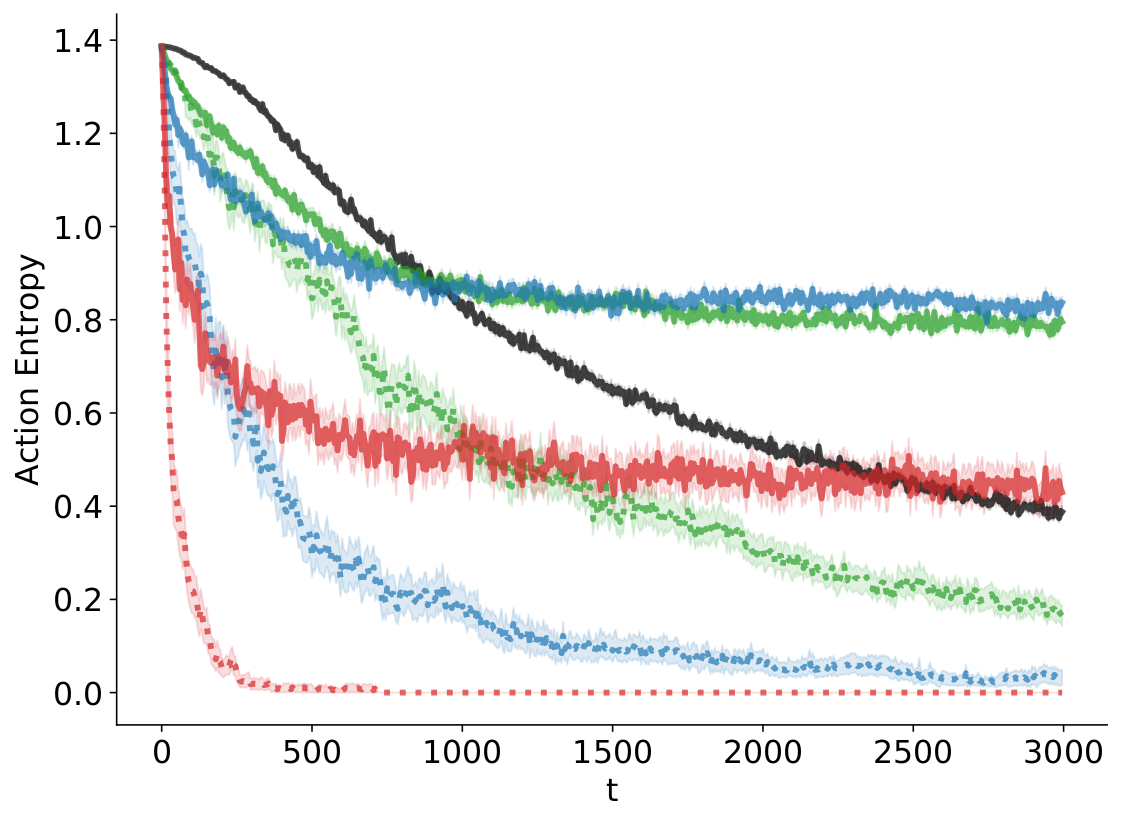
\includegraphics[width=\textwidth]{articles/baselines/figs/baseline_4rooms/NPG_action_entropy.png}
    \caption{Entropy (A)}
    \label{fig:4rooms_action}
  \end{subfigure}
  \begin{subfigure}[b]{0.25\linewidth}
    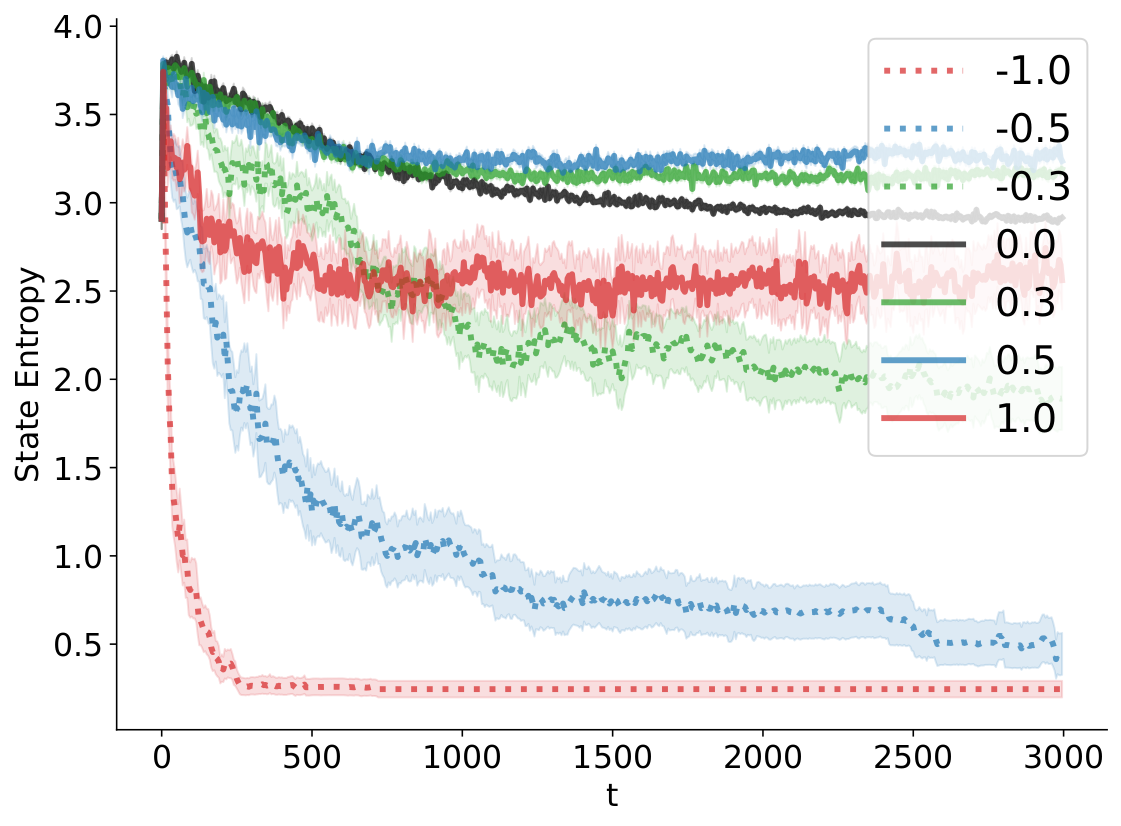
\includegraphics[width=\textwidth]{articles/baselines/figs/baseline_4rooms/NPG_state_entropy.png}
    \caption{Entropy (S)}
    \label{fig:4rooms_state}
  \end{subfigure}
  \caption{We plot the discounted returns, the entropy of the policy over the states visited in each trajectory, and the entropy of the state visitation distribution, averaged over 50 runs, for multiple baselines. The baselines are of the form $b(s) = b^*(s) + \epsilon$, perturbations of the minimum-variance baseline, with $\epsilon$ indicated in the legend. The shaded regions denote one standard error. Note that the policy entropy of lower baselines tends to decay faster than for larger baselines. Also, smaller baselines tend to get stuck on suboptimal policies, as indicated by the returns plot. See text for additional details.~\label{fig:stats_4rooms}}
\end{figure*}
We focused our theoretical analyses on multi-arm bandits so far. However, we are also interested in more general environments where gradient-based methods are commonplace. 
We now turn our attention to the Markov Decision Process (MDP) framework~\citep{puterman2014markov}. An MDP is a set $\{\gS, \gA, P, r, \gamma, \rho\}$ where $\gS$ and $\gA$ are the set of states and actions, $P$ is the environment transition function,
$r$ is the reward function, $\gamma \in [0, 1)$ the discount factor,
and $\rho$ is the initial state distribution. The goal of RL algorithms is to find a policy $\pi_\theta$, parameterized by $\theta$, which maximizes the (discounted) expected return; i.e. Eq.~\ref{eq:bandit_loss} becomes
\begin{align*}
    \arg\max_\theta \gJ(\theta)
    = \arg\max_\theta \sum_s d^{\pi_\theta}_\gamma(s)\sum_{a} \pi_\theta(a | s) r(s, a), %
\end{align*}
where there is now a discounted distribution over states induced by $\pi_\theta$. Although that distribution depends on $\pi_\theta$ in a potentially complex way, the parameter updates are similar to Eq.~\ref{eq:mc_update}:
\begin{align*}
    \theta_{t+1} &= \theta_t + \frac{\alpha}{N} \sum_i [Q(s_i, a_i) - b(s_i)]\nabla_\theta \log \pi_\theta(a_i | s_i) \label{eq:mc_update_mdp} \; ,
\end{align*}
where $(a_i, s_i)$ pairs are drawn according to the discounted state-visitation distribution induced by $\pi_\theta$ and $Q$ is the state-action value function induced by $\pi_\theta$~\citep[c.f.][]{sutton18book}. To match the bandit setting and common practice, we made the baseline state dependent. 

Although our theoretical analyses do not easily extend to multi-step MDPs, we empirically investigated if the similarity between these formulations leads to similar differences in learning dynamics when changing the baseline. We consider a 10x10 gridworld consisting of 4 rooms as depicted on Fig.~\ref{fig:4rooms_mdp}. We use a discount factor $\gamma=0.99$. The agent starts in the upper left room and two adjacent rooms contain a goal state of value $0.6$ or $0.3$. The best  goal (even discounted), with a value of $1$, lies in the furthest room, so that the agent must learn to cross the sub-optimal rooms and reach the furthest one. 

Similar to the bandit setting, for a state $s$, we can derive the minimum-variance baseline $b^*(s)$ assuming access to state-action values $Q(s,a)$ for $\pi_\theta$ and consider perturbations to it. Again, we use baselines $b(s) = b^*(s) + \epsilon$ and $b(s) = b^*(s) - \epsilon$, since they result in identical variances (this would not be the case if we used standard REINFORCE). 
We use a natural policy gradient estimate, which substitutes $\nabla \log \pi (a_i|s_i)$ by $F^{-1}_{s_i} \nabla \log \pi(a_i|s_i)$ in the update rule, where $F_{s_i}$ is the Fisher information matrix for state $s_i$ and solve for the exact $Q(s,a)$ values using dynamic programming for all updates (see Appendix \ref{app:npg_mdp_estimate} for details). 


In order to identify the committal vs. non-committal behaviour of the agent depending on the baseline, we monitor the entropy of the policy and the entropy of the stationary state distribution over time.
Fig.\ref{fig:4rooms_return} shows the average returns over time and Fig.\ref{fig:4rooms_action} and \ref{fig:4rooms_state} show the entropy of the policy in two ways. The first is the average entropy of the action distribution along the states visited in each trajectory, and the second is the entropy of the distribution of the number of times each state is visited up to that point in training.

The action entropy for smaller baselines tends to decay faster compared to larger ones, indicating convergence to a deterministic policy. This quick convergence is premature in some cases since the returns are not as high for the lower baselines.
In fact for $\epsilon=-1$, we see that the agent gets stuck on a policy that is unable to reach any goal within the time limit, as indicated by the returns of $0$.  
On the other hand, the larger baselines tend to achieve larger returns with larger entropy policies, but do not fully converge to the optimal policy as evidenced by the gap in the returns plot. 



Since committal and non-committal behaviour can be directly inferred from the PG and the sign of the effective rewards $R(\tau) - b$, we posit that these effects extend to all MDPs.
In particular, in complex MDPs, the first trajectories explored are likely to be suboptimal and a low baseline will increase their probability of being sampled again, requiring the use of techniques such as entropy regularization to prevent the policy~from~getting~stuck~too~quickly. 
In some preliminary experiments with a deep RL policy gradient algorithm, PPO \cite{schulman2017proximal}, where we perturb the baseline by a fixed constant, seem to indicate that negative perturbations perform slightly worse than positive perturbations. The results are not conclusive though and there are many confounding factors in this setting which could affect the outcome, including clipping due to PPO, neural network generalization, and adaptive optimizers. It is likely that a more careful strategy to perturb the baseline is needed to gain benefits, similar to using exploration bonuses. 

\section{Conclusion} 

We presented results that dispute common beliefs about baselines, variance, and policy gradient methods in general. 
As opposed to the common belief that baselines only provide benefits through variance reduction, we showed that they can significantly affect the optimization process in ways that cannot be explained by the variance and that lower variance can even sometimes be detrimental.

Different baselines can give rise to very different learning dynamics, even when they reduce the variance of the gradients equally. They do that by either making a policy quickly tend towards a deterministic one (\emph{committal} behaviour) or by maintaining high-entropy for a longer period of time (\emph{non-committal} behaviour). We showed that \textit{committal} behaviour can be problematic and lead to convergence to a suboptimal policy. Specifically, we showed that stochastic natural policy gradient does not always converge to the optimal solution due to the unusual situation in which the iterates converge to the optimal policy in expectation but not almost surely. 
Moreover, we showed that baselines that lead to lower-variance can sometimes be detrimental to optimization, highlighting the limitations of using variance to analyze the convergence properties of these methods. 
We also showed that standard convergence guarantees for PG methods do not apply to some settings because the assumption of bounded variance of the updates is violated.

The aforementioned convergence issues are also caused by the problematic coupling between the algorithm's updates and its sampling distribution since one directly impacts the other. As a potential solution, we showed that off-policy sampling can sidestep these difficulties by ensuring we use a sampling distribution that is different than the one induced by the agent's current policy. This supports the hypothesis that on-policy learning can be problematic, as observed in previous work~\citep{schaul2019ray, hennes2020neural}. Nevertheless, importance sampling in RL is generally seen as problematic~\citep{vanHasselt2018deadly_triad} due to instabilities it introduces to the learning process. Moving from an imposed policy, using past trajectories, to a chosen sampling policy reduces the variance of the gradients for near-deterministic policies and can lead to much better behaviour. In general, other variance-reduction strategies may also be more effective \cite{xu2019sample}.

More broadly, this work suggests that treating bandit and reinforcement learning problems as a black-box optimization of a function $\gJ(\theta)$ may be insufficient to perform well. As we have seen, the current parameter value can affect all future parameter values by influencing the data collection process and thus the updates performed. Theoretically, relying on immediately available quantities such as the gradient variance and ignoring the sequential nature of the optimization problem is not enough to discriminate between certain optimization algorithms. In essence, to design highly-effective policy optimization algorithms, it may be necessary to develop a better understanding of how the optimization process evolves over many steps. 


\section*{Acknowledgements}
We would like to thank Kris de Asis, Alan Chan, Ofir Nachum, Doina Precup, Dale Schuurmans, and Ahmed Touati for helpful discussions. We also thank Courtney Paquette, Vincent Liu, Scott Fujimoto and Csaba Szepesv\'{a}ri for reviewing an earlier version of this paper. Marlos C. Machado and Nicolas Le Roux are supported by a Canada CIFAR AI Chair.



